\section{Kebab shoarma z boczniaków z sałatką colesław i piklowaną cebulką}
\bigskip
\small
\begin{minipage}{0.45\textwidth}
    \noindent \textbf{Czas:} 30 minut \\
    \textbf{Poziom trudności:} łatwy
\end{minipage}
\begin{minipage}{0.45\textwidth}
    \noindent \textbf{Ilość sprzątania:} średnia\\
    \textbf{Wymagany mysi sprzęt:} -
\end{minipage}
\normalsize
\vspace{0.5cm}

\begin{multicols}{2}

\subsection*{Składniki}
\begin{itemize}
    \item 500 g boczniaków lub 150 g mięsa z kurczaka
    \item 2 łyżki oliwy
    \item 5 łyżek jogurtu greckiego
    \item 2 łyżki pasty tahini
    \item 1 cytryna
    \item 1/2 żółtej cebuli
    \item 1/4 czerwonej kapusty
    \item 1 łyżka majonezu
    \item przyprawa do kebaba shoarma lub gyrosa
    \item 2 łyżki sosu sojowego
    \item 1 łyżeczka pasty miso (opcjonalnie)
    \item ogórki kiszone lub korniszony
    \item chlebki pita
    \item sól i pieprz do smaku
\end{itemize}

\columnbreak

\begin{figure}[H]
    \centering
    \fbox{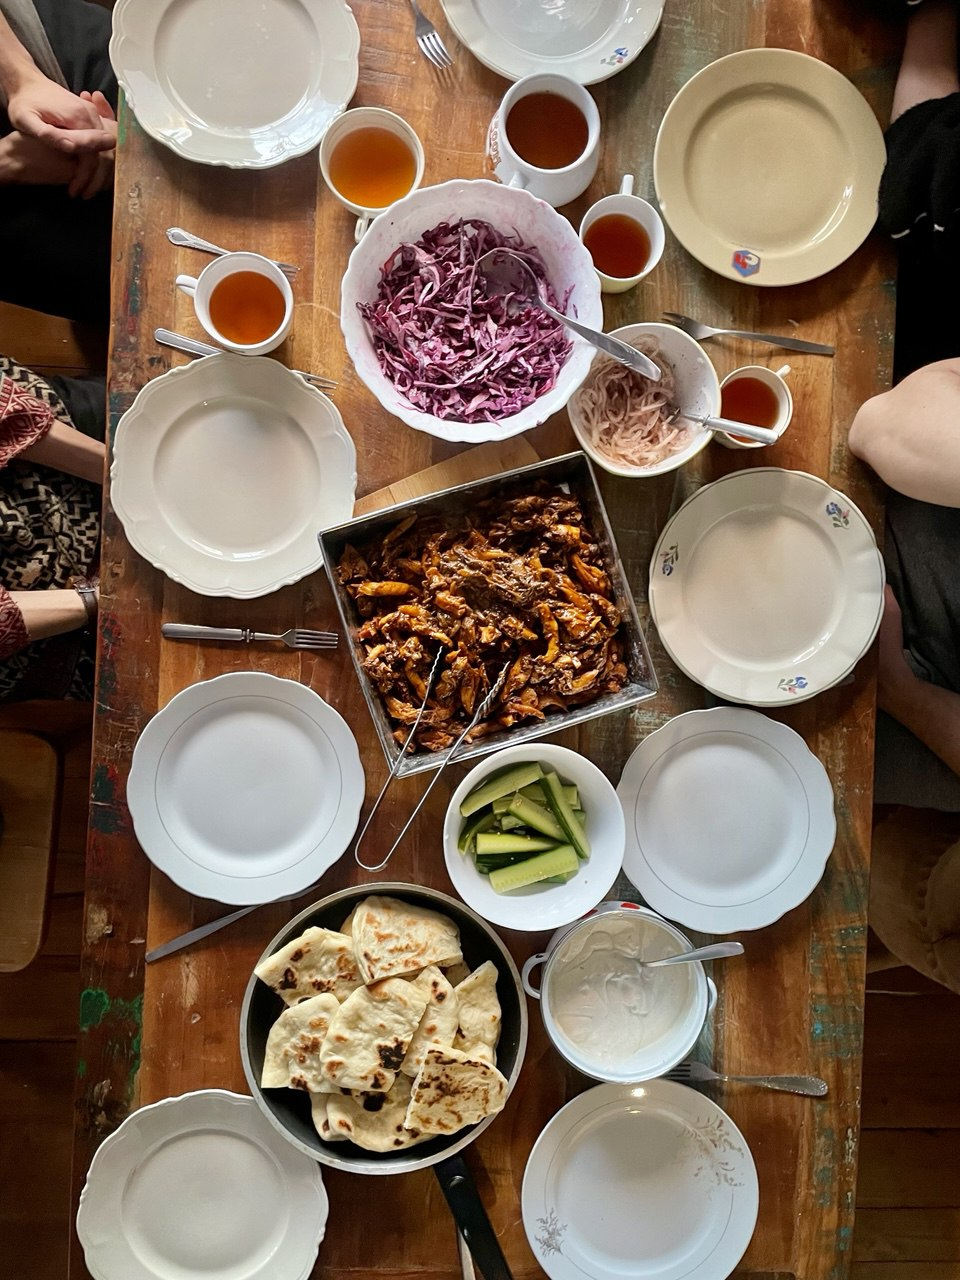
\includegraphics[width=0.4\textwidth]{images/kebabik.jpg}}
\end{figure}
\end{multicols}

\vspace{0.5cm}

\subsection*{Instruktaż}
\begin{enumerate}
    \item Grzyby oczyścić, a duże fragmenty przekroić lub porozdzielać rękami na mniejsze. Przełożyć do miski i zalać oliwą wraz z przyprawą, sosem sojowym i pastą miso. Wszystko dokładnie wymieszać i odstawić na 10 minut do zamarynowania.
    \item Cebulę pokroić w piórka, przełożyć do małej miseczki i wycisnąć do niej sok z połówki cytryny oraz doprawić solą oraz pieprzem. Wymieszać dokładnie palcami lub łyżeczką i odstawić na bok.
    \item Kapustę pokroić w piórka i wycisnąć do niej sok z połówki cytryny. Wymieszać. Dodać obfitą łyżkę majonezu, sporą szczyptę soli oraz pieprzu i wymieszać raz jeszcze.
    \item Do jogurtu dodać tahini oraz sól i pieprz do smaku.
    \item Rozgrzać mocno olej na średniej wielkości patelni. Boczniaki smażyć przez ok. 10 minut aż się skarmelizują. Boczniaki tracą mocno na objętości w trakcie smażenia, więc jeśli jest ich na początku za dużo, należy smażyć partiami.
    \item Chlebki pita podgrzać zgodnie z instrukcją na opakowaniu. Na ciepłe chlebki nałożyć sos, sałatkę colesław, boczniaki oraz ogórki. Udekorować piklowaną cebulką.
\end{enumerate}

\vspace{0.5cm}

\small
\subsection*{Propozycja podania}
Z chlebkami pita (domowe pity są dosyć łatwe w przygotowaniu) lub w tortilli.

\vspace{0.3cm}

\subsection*{Dodatkowe uwagi} W przepisie zamiast sosu tahini równie dobrze sprawdza się domowej roboty sos czosnkowy.
